\begin{figure}[htbp]
\section*{ ATP13A2}
\centering
\begin{subfigure}[b]{0.95\textwidth}
\centering
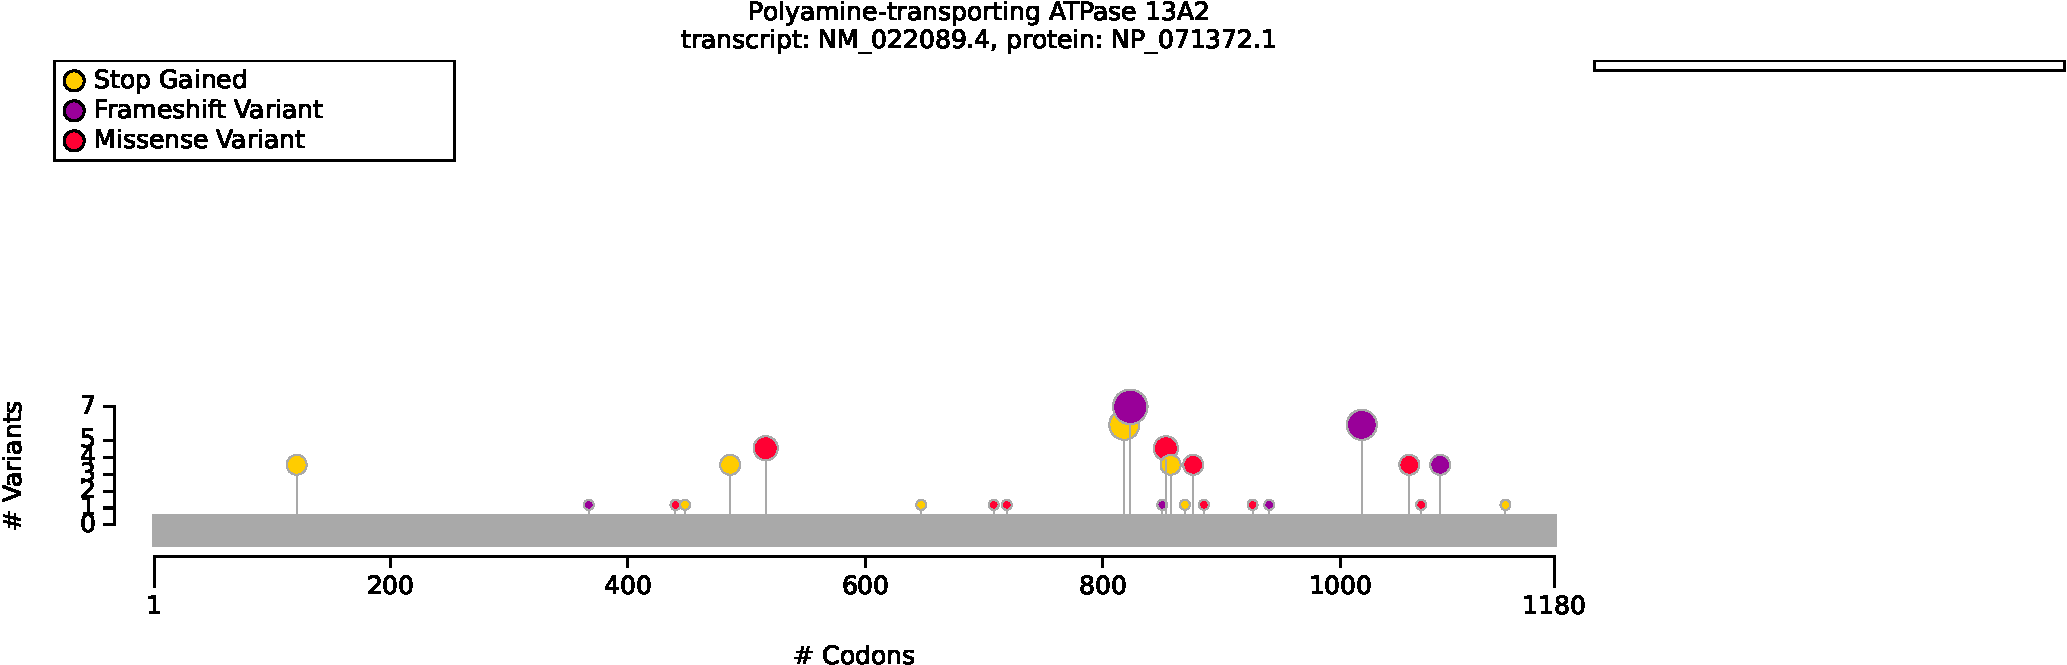
\includegraphics[width=\textwidth]{ img/ATP13A2_protein_diagram.pdf} 
\captionsetup{justification=raggedright,singlelinecheck=false}
\caption{Distribution of variants in ATP13A2}
\end{subfigure}

\vspace{2em}

\begin{subfigure}[b]{0.95\textwidth}
\centering
\resizebox{\textwidth}{!}{
\begin{tabular}{llllrr}
\toprule
HPO term & OMIM:606693 & OMIM:617225 & p-value & adj. p-value\\
\midrule
Parkinsonism [HP:0001300] & 28/28 (100\%) & 3/11 (27\%) & $2.68\times 10^{-6}$ & $7.78\times 10^{-5}$\\
Bradykinesia [HP:0002067] & 30/32 (94\%) & 4/10 (40\%) & $9.15\times 10^{-4}$ & 0.013\\
\bottomrule
\end{tabular}
}
\captionsetup{justification=raggedright,singlelinecheck=false}
\caption{Fisher Exact Test performed to compare HPO annotation frequency with respect to 
Kufor-Rakeb syndrome (OMIM:606693) and Spastic paraplegia 78, autosomal recessive (OMIM:617225).
Total of 29 tests were performed. }
\end{subfigure}
\vspace{2em}
\begin{subfigure}[b]{0.95\textwidth}
\centering
\resizebox{\textwidth}{!}{
\begin{tabular}{llllrr}
\toprule
Genotype (A) & Genotype (B) & total tests performed & significant results\\
\midrule
missense/missense OR missense/other & other/other & 30 & 0\\
\bottomrule
\end{tabular}
}
\captionsetup{justification=raggedright,singlelinecheck=false}
\caption{Fisher Exact Test performed to compare HPO annotation frequency with respect to genotypes.}
\end{subfigure}

\vspace{2em}

\caption{The cohort comprised 45 individuals (18 females, 27 males). A total of 71 HPO terms were used to annotate the cohort. 
Disease diagnoses: Kufor-Rakeb syndrome (OMIM:606693) (34 individuals), Spastic paraplegia 78, autosomal recessive (OMIM:617225) 
(11 individuals). As expected, the frequency of Parkinsonian manifestations is higher in Kufor-Rakeb syndrome,
 a rare autosomal recessive form of juvenile-onset atypical Parkinson disease. A total of 24 unique variant alleles were found in \textit{ATP13A2} (transcript: \texttt{NM\_022089.4}, protein id: \texttt{NP\_071372.1}).}
\end{figure}
